\documentclass{article}[18pt]
\usepackage{../../../../format}
\lhead{Networks and Systems - Compiler Design}


\begin{document}
\begin{center}
\underline{\huge Introduction}
\end{center}
\section{Languages}
\subsection{Natural Languages}
Natural languages have:
\begin{itemize}
	\item Words
	\item Types of words
	\item Syntax
	\item Meaning of words (semantics)
\end{itemize}
Natural languages are useful for communication between humans, but only if they speak the same language, otherwise we need translation
\subsection{Programming Languages}
Communication between humans and computers can't be done by default as a human speaks a natural language and a computer "speaks" machine languages.\\
\\
The solution to this:
\begin{itemize}
	\item Using a programming language
	\item Understandable by humans
	\item But much more structured than natural languages
	\item But still very far from being "machine" language
\end{itemize}
\section{Compilers}
We need a way to write something in some programming language and "translate" it into executable machine language\\
\\
Compiler: a computer program that transforms:
\begin{itemize}
	\item A program, written in a programming language (source program/source language)
	\item To an equivalent program in another language (target program/target language)
\end{itemize}
Any language can be a target language.\\
\\
The most common target program is an executable machine-language program
\section{Compilers vs Interpreters}
\subsection{Compilers}
After compilation, the target program:
\begin{itemize}
	\item Is called by the user
	\item Processes input and produces output
\end{itemize}
\begin{center}
	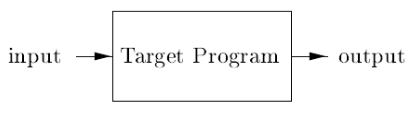
\includegraphics[scale=0.7]{Compiler}
\end{center}
\subsection{Interpreters}
Directly executes the operations specified in the source program on inputs supplied by the user
\begin{center}
	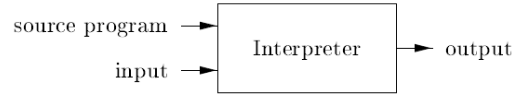
\includegraphics[scale=0.7]{Interpreter}
\end{center}
\subsection{Comparison}
While mapping input to output:
\begin{itemize}
	\item The machine-language target program (built by a compiler) is faster
	\item An interpreter gives better error diagnostics (it executes the source program statement by statement)
\end{itemize}
\section{Compilers}
Compilers and interpreters must:
\begin{itemize}
	\item Detect lexical/syntactic/semantic inconsistencies 
	\item Propose solutions wherever possible
\end{itemize}
\subsection{Structure of a compiler}
Analysis part (front end)
\begin{itemize}
	\item Breaks the source program into constituent pieces
	\item Imposes grammatical structure on them (according to the rules of the source language)
	\item Creates intermediate representation (IR) of the source program
	\item Provides informative error messages (if errors detected)
	\item Collects all the important information in a symbol table and passes the symbol table and IR along to the synthesis part
\end{itemize}
Synthesis part (back end)
\begin{itemize}
	\item Uses the symbol table and the IR
	\item Generates and optimises the target code
\end{itemize}
Main phases of the analysis part
\begin{itemize}
	\item Lexical analysis (scanning)
	\item Syntax analysis (parsing)
	\item Semantic analysis
\end{itemize}
Main phases of the synthesis part
\begin{itemize}
	\item Target code generation
	\item Target code optimization
\end{itemize}
\subsection{Strict separation}
Why separate analysis and synthesis parts?
\begin{itemize}
	\item Can combine different analysis/synthesis parts in a modular way
	\item Create new compilers
	\item For L languages and M machines
	\begin{itemize}
		\item We need only L+M modules instead of $L\times M$
	\end{itemize}
\end{itemize}
\section{Internal phases of a compiler}
\subsection{Lexical analysis/scanning}
\begin{itemize}
	\item Reads the input program as a character stream
	\item Groups the characters into meaningful sequences (lexemes)
	\begin{center}
		position=initial + rate * 60
	\end{center}
	\item For each lexeme creates a tone (acts as one single symbol)
	\begin{center}
		$\langle id,1\rangle \langle = \rangle \langle id,2 \rangle \langle + \rangle \langle id,3 \rangle \langle * \rangle \langle 60 \rangle$
	\end{center}
\end{itemize}
\subsection{Syntax analysis/Parsing}
\begin{itemize}
	\item Uses the tokens from the lexical analysis
	\item Creates a tree like intermediate representation of the source program
	\item Syntax tree/parse tree
	\begin{itemize}
		\item Interior nodes: operations
		\item Children nodes: arguments of the operations
	\end{itemize}
\end{itemize}
\begin{center}
	\includegraphics[scale=0.5]{"Parse Tree"}
\end{center}
\subsection{After syntax analysis}
All the subsequent phases use:
\begin{itemize}
	\item The symbol table (i.e. all the parts of the source program)
	\item The syntax tree (i.e. the grammatical structure of the program)
\end{itemize}
In order to:
\begin{itemize}
	\item Analyse further the program
	\item Produce the target code
\end{itemize}
\subsection{Semantic analysis}
\begin{itemize}
	\item Uses the symbol table and syntax tree
	\item Checks for semantic consistency with the source language definition
	\item Stores the semantic information in the symbol table or the syntax tree (for further use)
	\item Important part is type checking and automatic type conversion (coercion)
\end{itemize}
\begin{center}
	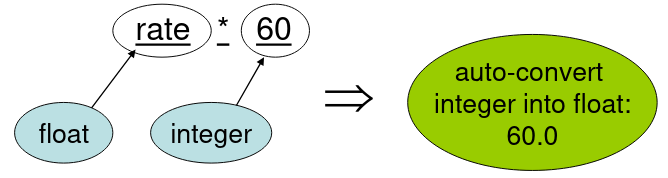
\includegraphics[scale=0.7]{Coercion}
\end{center}
\subsection{Intermediate code generation}
\begin{itemize}
	\item Explicit low-level machine-like code
	\item It must be easy to both produce and to translate into target machine code
	\item Usually a tree address code
	\begin{itemize}
		\item Simple instructions
		\item Three operands per instruction
	\end{itemize}
\end{itemize}
\begin{center}
	\includegraphics[scale=0.7]{"Intermediate Code"}
\end{center}
\subsection{Intermediate code optimization}
\begin{itemize}
	\item Improve the intermediate code into a "better" code
	\item Better can be
	\begin{itemize}
		\item Faster
		\item Shorter
		\item Consume less power
	\end{itemize}
\end{itemize}
\begin{center}
	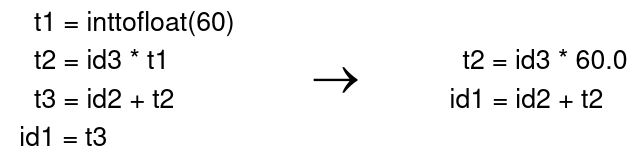
\includegraphics[scale=0.7]{optimization}
\end{center}
\section{Symbol table management}
Store in symbol table (except variable names):
\begin{itemize}
	\item Attributes with additional information, e.g.:
	\begin{itemize}
		\item Type
		\item Storage address
		\item Scope (where in the program the value is used)
	\end{itemize}
	\item Also, for the case of procedure names:
	\begin{itemize}
		\item Number and types of its arguments
		\item Method of passing each argument (value or reference)
	\end{itemize}
\end{itemize} 
\section{Passes}
In practice, phases of the compiler may be "grouped" together in passes
\section{Evolution of compilers}
Generations of programming languages
\begin{itemize}
	\item 1st generation - 0s and 1s
	\item 2nd generation - assembly languages
	\item 3rd generation - higher level (Java, C)
	\item 4th generation - specific applications (SQL)
\end{itemize}
Can use previous compilers for new languages\\
T diagrams: a set of "puzzle pieces"
\begin{center}
	\includegraphics[scale=0.7]{"T Diagram"}
\end{center}
Recursive use of compilers (and T diagrams):
\begin{itemize}
	\item 1st compiler written in S translating A to T
	\item 2nd compiler written in T translating S to T
	\item Third compiler written in T translating A to T
\end{itemize}
\begin{center}
	\includegraphics[scale=0.7]{"Recursive Compiler"}
\end{center}


\end{document}